% If you want to compile this section only, make sure to include relevant document headers and the \being \end document commands.
% You can make this a bit easier if you use the subfile package

As my MA thesis, this topic is highly feasible. About the technical skills, I am the right researcher for this project. Firstly, I am familiar with both GIS and commercial real estate. I was trained as a GIS geographer during my undergraduate study. Besides that, I have four years of work experience practicing GIS in commercial real estate and one year of technical support experience in GIS software. I have the adequate technical background and data visualization skills needed for the GIS part of my research design. Secondly, regarding the statistics part of this research, which is to apply the hedonic regression model, I plan to take statistics classes with Professor Yanyan Sheng in the quarters to come, to get familiar with different statistic models and methodologies. Thirdly, Professor Crystal Bae from the Center for Spatial Data Science read through my literature review on spatial cognition and provided helpful suggestions. She also agreed to provide further guidance and suggestions during my research implementation.

Regarding data availability and data security, as discussed in the Research Design and Data Collection/Preparation part, both satellite imagery lidar data and housing data are publicly available through USGS and Redfin. USGS provides data access to the public, so downloading data from the website of USGS should be easy. Although Redfin prohibits web scraping private data in their terms of use, extracting publicly available information about the listings is legal. Since the information I will collect for the research design is public to everyone. There should not be any problems with the accessibility and utilization of Redfin data. 

Finally, regarding IRB reviews, this project does not contain human subjects. I do not interact with human individuals during data collection. What is more, the research design shows significant social beneficence. Understanding the relationship between UGS and housing prices can help us better understand the importance of UGS and its economic benefits. It can also provide substantial proof that encourages city governors and urban planners to incorporate more minor UGS. Together, we can utilize UGS to improve social justice by creating an urban environment that is friendly to all.

I am at the end of Spring Quarter 2024. I plan to use the next four quarters to continue working on my thesis. Please refer to the following graph for timeline information (Figure 5).

\begin{figure}[h]
    \centering
    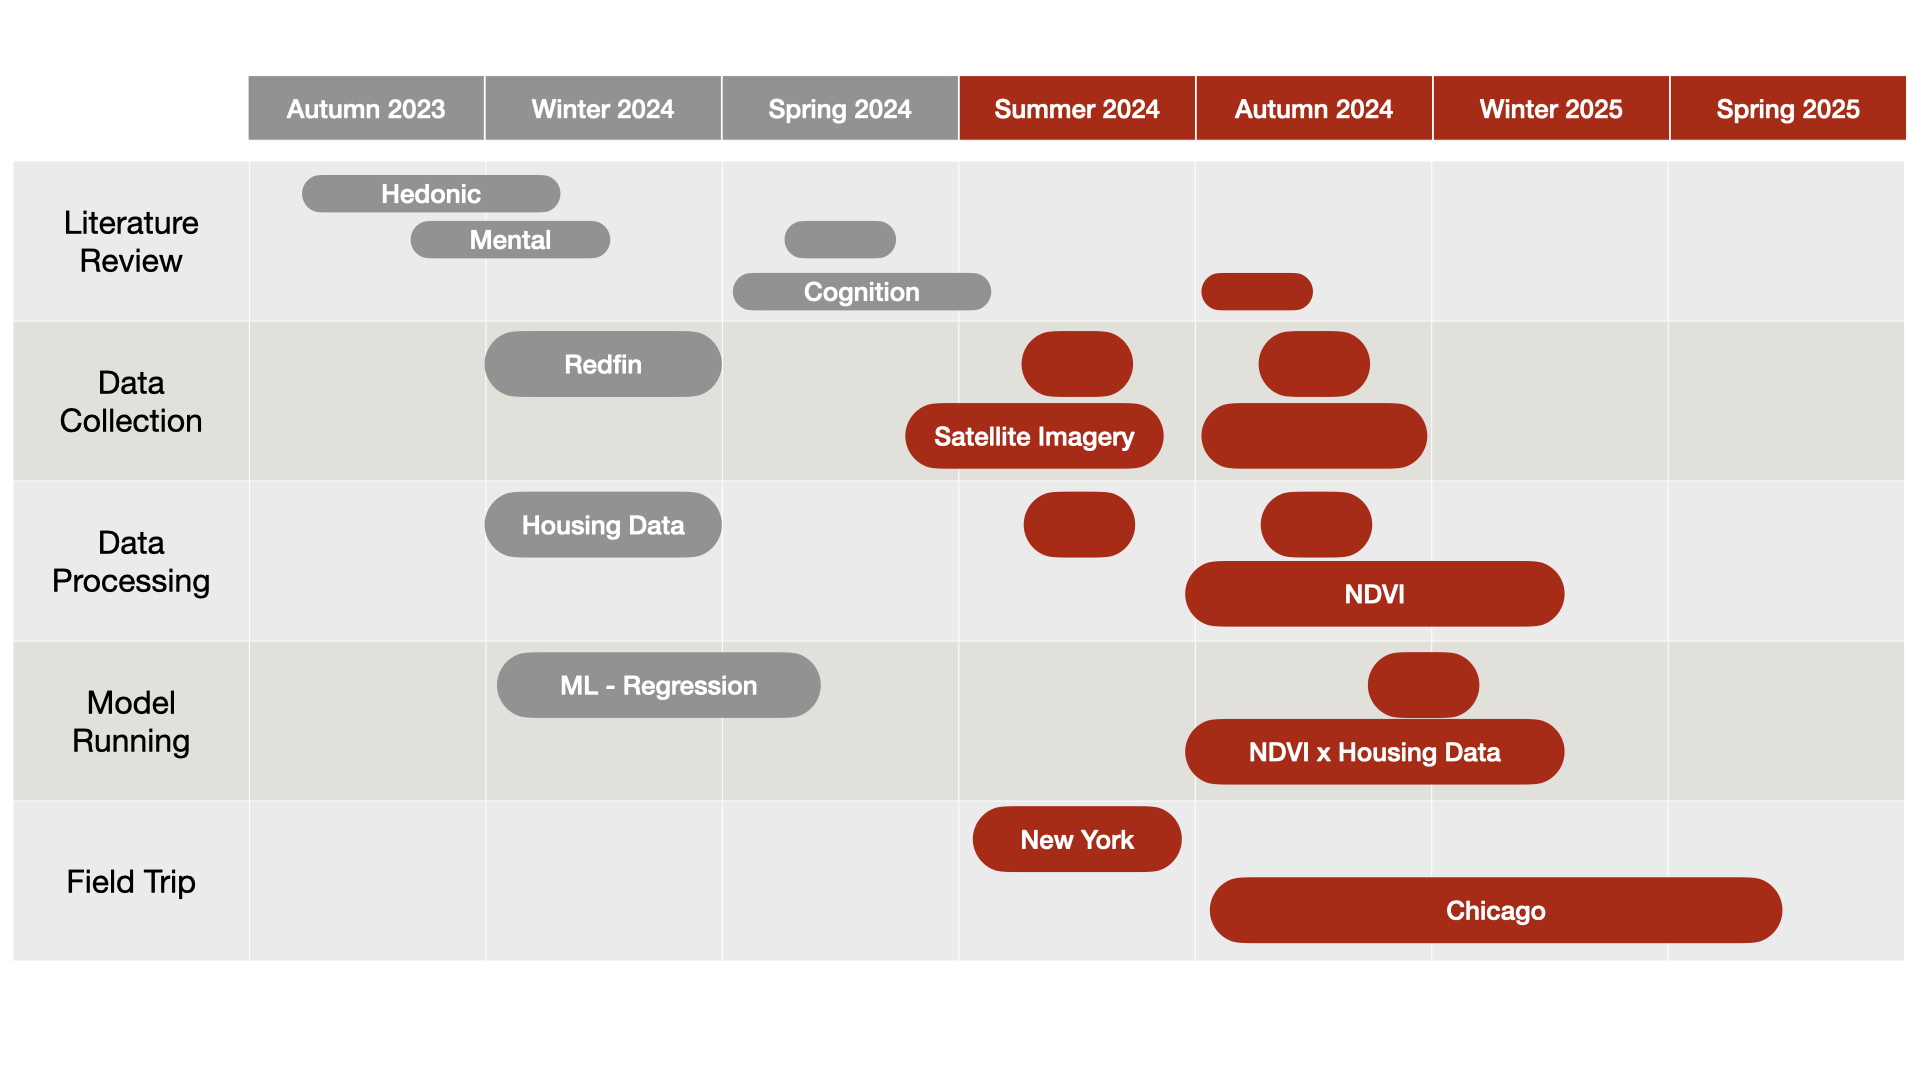
\includegraphics[width=1\textwidth]{Visual/final_timeline.jpeg}
    \caption{Proposed Timeline}
\end{figure}